\documentclass[../sparc.tex]{subfiles}
\graphicspath{{\subfix{../images/}}}
\begin{document}

%%%%%%%%%%%%%%%%%%%%%%%%%%%%%%%%%%%%%%%%%%%%%%%%%%%%%%%%%%%%%%%%%%%%%%%%%%%%%%%%
\section{Serial Port}
\index{Electronics!Serial Port}
\label{section:serial-port}

Connection of Arduino to a computer is usually is done through a USB connector
placed on the board.  On the Arduino Mega 2560 side USB-B is used for that
purpose.

The USB protocol is quite complicated and the most of the Arduino chips don't
``speak'' USB protocol and need a ``translator'' to be understood by a computer.
A translator is usually a separate chip called USB-UART converter soldered on an
Arduino board.  We will discuss UART in a section
\ref{section:communication-uart}.  Some compact Arduino such as Arduino Pro Mini
does not have its own USB-UART converter and require a separate converter.

An USB-UART converter emulates a simpler data transfer protocol than USB that is
commonly known as ``Serial Port''.  On old computers this port (also known as
COM-port) was represented as a separate interface on the main board and was used
to connect such devices as computer mice.  COM-ports used to be quite widespread
back in the days (for example they were popular on IBM PC AT computers.)  In the
modern world COM-ports were replaced in most of the consumer electronics with
other standards, mostly USB.  But COM-ports are still in use today on
specialized equipment.

One of the examples where serial ports are used to this day is working with
microcontrollers.  USB-UART converter emulates a COM-port for a computer
allowing to ``communicate'' with a microcontroller using a simpler language than
USB.  Thus for a computer an Arduino looks like a COM-port despite that the
physical connection is done through a USB.  Using this line of communication we
can transfer data from a computer to an Arduino and vice versa.

We will discuss serial ports in more detail in the section
\ref{section:communication-serial-port}.  Currently we only need the basic
knowledge on this topic in order to understand the examples in chapter.

%%%%%%%%%%%%%%%%%%%%%%%%%%%%%%%%%%%%%%%%%%%%%%%%%%%%%%%%%%%%%%%%%%%%%%%%%%%%%%%%
\subsection{Basics of Serial Port Usage in Arduino}

Before we start working with a serial port we need to configure it.  It can be
done as follows: first we need to configure the speed of data transfer in
\texttt{setup} function:

\begin{minted}{cpp}
  void setup() {
    Serial.begin(9600);
  }
\end{minted}

In this case we are allowing data transfer between a computer and an Arduino
with the specified speed where 9600 is the speed set in \emph{bauds}.  A
\emph{baud} is a unit of data transfer speed measurement that is equal to a bit
per second.  Usually this parameter is set to one of the standard values: 300,
600, 1200, 2400, 4800, 9600, 14400, 19200, 28800, 38400, 57600, 115200.

%%%%%%%%%%%%%%%%%%%%%%%%%%%%%%%%%%%%%%%%%%%%%%%%%%%%%%%%%%%%%%%%%%%%%%%%%%%%%%%%
\subsection{Transferring Data to a Computer}

Now let's try to transfer some data to a computer.  As the first example we will
send ``Hello, world!'' string through a serial port.  First we need to write
down the serial port configuration in the \texttt{setup} function:

\begin{minted}{cpp}
  void setup() {
    Serial.begin(9600); // Setting the speed of a serial port.
  }
\end{minted}

And that's how our \texttt{loop} function looks like:

\begin{minted}{cpp}
  void loop() {
    Serial.println("Hello World");
    delay(1000); // Waiting 1000 ms before the next transfer
  }
\end{minted}

To see the results of program execution we need to open the ``Serial Monitor''
in the Arduino IDE from the ``Tools'' menu.

Aside from that we can open ``Serial Monitor'' by \hotkey{Ctrl + Shift + M}
hotkey.

\begin{figure}[ht]
  \centering
  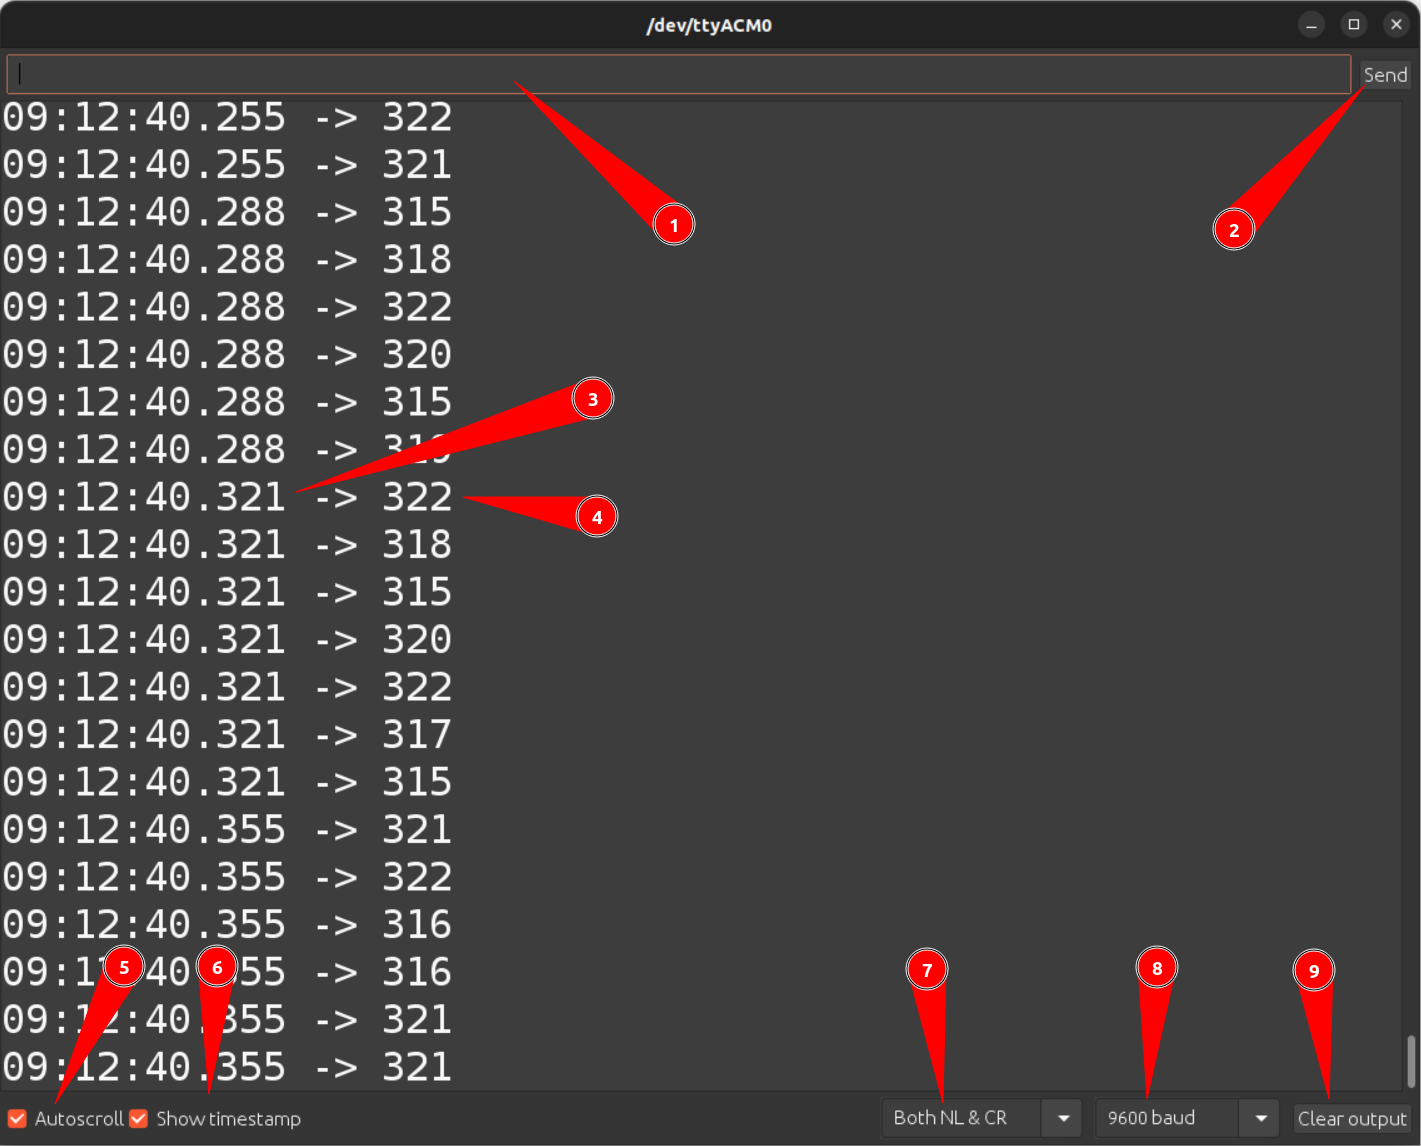
\includegraphics[width=10cm]{arduino-ide-serial-monitor}
  \caption{``Serial Monitor'' in Arduino IDE 1.8.19.}
  \label{fig:arduino-ide-serial-monitor}
\end{figure}

The overall view of the serial monitor is shown on fig.
\ref{fig:arduino-ide-serial-monitor}.  In the window header we can see the name
of the device that represents an connected Arduino.  This device is used by your
computer to talk to the Arduino.

Also you can see an input field below the window header that is used to send
data to the Arduino board.

The main area of the window is taken by the area that shows the data that is
received from the Arduino.

In the bottom of the window the configuration panel is located.

The numbers on the fig. \ref{fig:arduino-ide-serial-monitor} show:
\begin{enumerate}
\item An input field for sending data from a computer to an Arduino.
\item ``Send'' button that sends data from the input field on the left to an
  Arduino.
\item Timestamp that marks the moment when the data was received on the
  computer.
\item The data that was received from an Arduino.
\item ``Autoscroll'' option.  If this option is enabled then the main area of
  the window that shows the received data is scrolled automatically in such way
  so it always shows the latest data tat was received.
\item ``Show timestamp'' option that allows us to enable timestamps (as is the
  \textbf{3} on the picture.)
\item An option that controls the line endings in the communication with an
  Arduino.  This option controls which sequence of symbols the serial monitors
  considers as a line ending.  You can choose from ``No line ending'',
  ``Newline'', ``Carriage return'' and ``Both NL \& CR'' (when this mode is
  enabled two symbols are used together -- a newline and a carriage return.)
\item An option that controls the speed of data transfer in bauds (bits per
  second.)  This is set to 9600 by default.  If the option value is not matching
  the value in the program on an Arduino (through \texttt{Serial.begin}) then
  the serial monitor will show garbage symbols instead of correct data.
\item ``Clear output'' button that allows us to clear the main area of the
  window from the old data that was received from an Arduino.
\end{enumerate}

Data transfer between an Arduino and a computer can be used for many different
tasks.  For example one of such tasks is the simple way to debug your programs
on the Arduino board by simply printing various information about the runtime
program state through the serial port.  In other words instead of trying to
figure out the what the program does we can instruct an Arduino board to tell us
what it does.

%%%%%%%%%%%%%%%%%%%%%%%%%%%%%%%%%%%%%%%%%%%%%%%%%%%%%%%%%%%%%%%%%%%%%%%%%%%%%%%%
\subsection{Data Visualization}

In case of big amounts of data it becomes inconvenient to watch it in ``Serial
Monitor'' -- can get overwhelmed quite soon from the avalanche of numbers.  In
such situations data visualization can be of a great help for us.

Data visualization is an important component of data analysis: graphical
representation of featureless numbers allows us to quickly and capaciously grasp
the information with just one look.  And often this helps us to see regularities
in the data that can be hidden from the eye in other cases.

There are different ways to visualize the data; one of such possibilities that
is available for us is ``Serial Plotter'' that allows us to get a graph from the
incoming data right from the Arduino IDE.  We can access the plotter through
``Tools'' menu wehre we have to select ``Serial Plotter'' (or we can use
\hotkey{Ctrl + Shift + L} hotkey to access the plotter.)

The overall appearance of the plotter is shown on
fig. \ref{fig:arduino-ide-serial-plotter}.

As for the serial monitor the header of the plotter shows the name of the device
that represents an Arduino device connected to the computer.

\begin{figure}[ht]
  \centering
  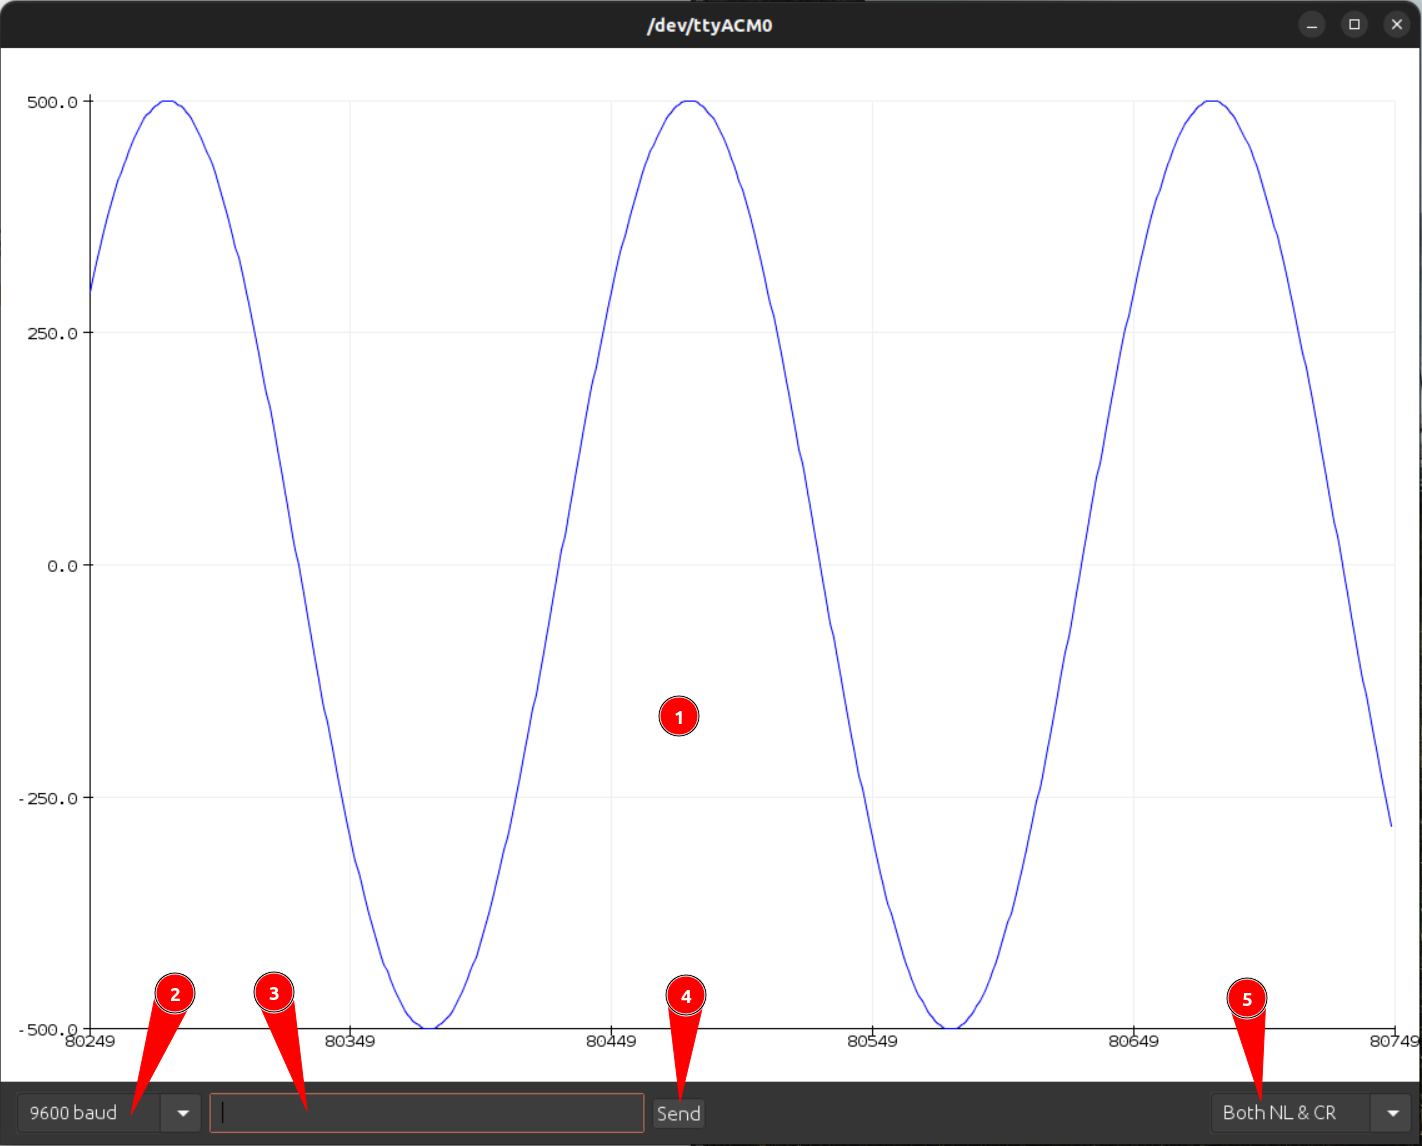
\includegraphics[width=10cm]{arduino-ide-serial-plotter}
  \caption{Плоттер по последовательному соединению (``Serial Plotter'') в
    Arduino IDE 1.8.19.}
  \label{fig:arduino-ide-serial-plotter}
\end{figure}

The numbers on fig. \ref{fig:arduino-ide-serial-plotter} show:

\begin{enumerate}
\item The area of graph view where the incoming data from an Arduino is shown.
\item A drop-down menu that allows us to configure the speed of serial port in
  bauds (bits per second.)  This is set to 9600 baud by default.  If this
  parameter value differs from the serial port speed configured in the Arduino
  program (through \texttt{Serial.begin}) then the plotter will not be able to
  show the data.
\item Data input line that allows us to send data from a computer to the
  connected Arduino.
\item ``Send'' button that when clicked initiates the data transfer from the
  input line one the left to the button to the connected Arduino.
\item Line ending configuration for the Arduino communication.  There we can
  choose one of the following modes: ``No line ending'', ``Newline'', ``Carriage
  return'' and ``Both NL \& CR'' (the mode where both ``Newline'' and ``Carriage
  return'' is used.)  This option configures which sequence of symbols is used
  as the line eding.
\end{enumerate}

\newpage

By the way the sine wave that is shown on fig.
\ref{fig:arduino-ide-serial-plotter} is generated by the following code:

\begin{listing}[ht]
  \begin{minted}{cpp}
    void setup() {
      Serial.begin(9600);
    }

    int t = 0;
    void loop() {
      const double AMPLITUDE = 500;
      double y = AMPLITUDE * sin(2.0 * PI / 200 * t);
      Serial.println(y);
      t++;
      delay(1);
    }
  \end{minted}
  \label{listing:serial-port-sine-wave-example}
  \caption{An example of a program for Arduino that generates a sine wave in the
    serial plotter on a computer.}
\end{listing}

\subsection{Transferring Data from a Computer}

At this moment we know how to transfer data from an Arduino to a computer. Now
let's take a look on the data transferring in the reverse direction. To transfer
some data from a computer to an Arduino we have to configure the serial port as
in previous examples.  Aside from that we will need to learn some new functions.

\subsubsection{Reading Bytes}

\texttt{Serial.read} function reads one byte of data from the serial port on an
Arduino.  In other words it returns us some number as the result that we can use
as we wish.  Each call to \texttt{Serial.read} returns the next byte from the
serial port.  If there's no data to read (that is, when you read all the data)
the function returns -1 as the value.

\note{To make sure that we have some data to read we can call
  \texttt{Serial.available} function that returns the number of bytes available
  for reading.}

Let's assume that we have sent 1 byte of data to an Arduino and use the
following piece of code to handle it:

\begin{minted}{cpp}
  int incoming_byte;
  void loop() {
    if (Serial.available() > 0) {
      incoming_byte = Serial.read();
    }
  }
\end{minted}

After we read a byte of data it will be saved into our variable
\texttt{incoming\_byte} and \texttt{Serial.available} will return 0 until new
data is available.

In other words when you read a byte the counter of the received bytes will
decrease and \texttt{Serial.available} when called will return one byte less.

Remember that \texttt{Serial.read} returns only one byte of data and if you, for
example, have sent 4 symbols each 1 byte long then you have to call
\texttt{Serial.read} four times to read all the symbols.

\end{document}
